\section{Abstract}
Dieser Versuch beschäftigt sich mit der optischen Fouriertransformation eines Laserstrahls an einem Objekt und den Möglichkeiten, die sich daraus ergeben. Zuerst wird das Interferenzbild eines Gitters in unterschiedlichen Entfernungen betrachtet, um so den Übergang von der Fresnel- zur Fraunhoferbeugung darzustellen. Anschließend werden die Gitterkonstanten fünf verschiedener Gitter auf zwei verschiedene Arten bestimmt, zuerst ohne Linse, anschließend mit einer Sammellinse.

Die Gitterkonstanten stimmen bei beiden Versuchsaufbauten überein, nur Gitter 1 wurde bei einer Messung offenbar falsch bestimmt. Die Methoden sind also beide gut zur Bestimmung der Gitterkonstanten geeignet.


Als letztes werden Hoch- und Tiefpassfilter benutzt, um verschiedene Bildeffekte zu erzeugen. Insgesamt konnten alle Effekte gezeigt werden, allerdings wurden die Filter nicht immer perfekt in der Fourierebene abgestellt, weshalb die erzeugten Bilder zum Teil auch ungewollte Effekte aufzeigen. 




\section{Theorie}
Dieses komplette Kapitel wurde aus \autocite{anleitung-ws2014} zusammengefasst
\subsection{Fouriertransformation}
Die Fouriertransformation wird in der Signalverarbeitung verwendet, um Signale in den Frequenzraum und zurück zu transformieren. Dabei können sowohl zeitliche Signale in ihre zeitlichen Frequenzen zerlegt werden, als auch räumliche Signale in ihre räumlichen Frequenzen. \cref{eq:tfourier} zeigt die Gleichung für die Umwandlung zeitlicher Signale, \cref{eq:xyfourier} zeigt die Gleichung für die Umwandlung zweidimensionaler räumlicher Signale.

\begin{equation}
	\mathcal{F}\left[ f\left( t\right) \right] \left( \nu\right) = \frac{1}{\sqrt{2\pi}} \int_{-\infty}^{\infty} f\left( t\right) e^{-2\pi i \nu t} \text{d}t = F\left( \nu\right) 
	\label{eq:tfourier}
\end{equation}

\begin{equation}
	\mathcal{F}\left[ f\left( x,y\right) \right] \left( \nu_x, \nu_y\right) = \frac{1}{\sqrt{2\pi}} \int_{-\infty}^{\infty} \int_{-\infty}^{\infty} f\left( x, y\right) e^{-2\pi i (\nu_x x + \nu_y y)} \text{d}x \text{d}y = F\left( \nu_x, \nu_y\right) 
	\label{eq:xyfourier}
\end{equation}

Dabei sind $F\left( \nu\right)$ bzw. $F\left( \nu_x, \nu_y\right)$ die Funktion im Frequenzraum, $f\left( t\right)$ die Funktion im Zeitraum, $f\left( x,y\right)$ die Funktion im Ortsraum, $t$ die Zeit, $x$ und $y$ die räumlichen Koordinaten, $\nu$ die zeitliche Frequenz und $\nu_x$ und $\nu_y$ die räumlichen Frequenzen. Die jeweiligen Rücktransformationen werden durch \cref{eq:trück}(zeitlich) und \cref{eq:xyrück}(räumlich) beschrieben.

\begin{equation}
	\mathcal{F}^{-1}\left[ f\left( \nu\right) \right] \left( t\right) = \frac{1}{\sqrt{2\pi}} \int_{-\infty}^{\infty} F\left( \nu\right) e^{-2\pi i \nu t} \text{d}\nu = f\left( t\right) 
	\label{eq:trück}
\end{equation}

\begin{equation}
	\mathcal{F}^{-1}\left[ f\left( \nu_x,\nu_y\right) \right] \left( x, y\right) = \frac{1}{\sqrt{2\pi}} \int_{-\infty}^{\infty} \int_{-\infty}^{\infty} F\left( \nu_x,\nu_y\right) e^{-2\pi i (\nu_x x + \nu_y y)} \text{d}\nu_x \text{d}\nu_y = f\left( x, y\right) 
	\label{eq:xyrück}
\end{equation}

Ein Beispiel für die Fouriertransformation ist in \cref{rechteckpuls} dargestellt. Dort ist ein Rechteckpuls und seine Fouriertransformierte, eine sinc-Funktion, in einer Dimension dargestellt. 

\begin{figure}[h!]
	\centering
	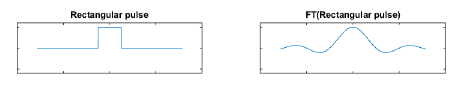
\includegraphics[width=0.9\textwidth]{rechteckpuls.PNG}
	\caption{Fouriertransformation, angewandt auf einen Rechteckpuls. Das Ergebnis ist eine sinc-Funktion. Entnommen aus \autocite{anleitung-ws2014}}
	\label{rechteckpuls}
\end{figure}

Bei der optischen Fouriertransformation ist allerdings eine Transformation in zwei räumlichen Dimensionen nötig. Dies ist in \cref{rechteckspalt} dargestellt. Hier wird ein Rechteckspalt fouriertransformiert, heraus kommen eine sinc-Funktion in x- und eine sinc-Funktion in y-Richtung, die sich überlagern.

\begin{figure}[h!]
	\centering
	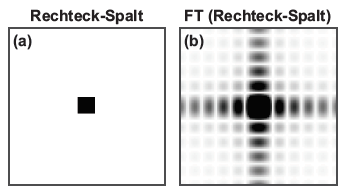
\includegraphics[width=0.7\textwidth]{rechteckspalt.PNG}
	\caption{Ein Rechteckspalt und die Fouriertransformierte, zwei sich überlagernde sinc-Funktionen. Entnommen aus \autocite{anleitung-ws2014}}
	\label{rechteckspalt}
\end{figure}

Die Fouriertransformation ist außerdem ein nützliches Werkzeug, um die Faltung zweier Funktionen zu beschreiben. Diese wird häufig verwendet, um periodische Strukturen wie Gitter zu beschreiben. Die Faltung ist im Orts- bzw. Zeitraum ein kompliziert zu bestimmendes Integral. Allerdings ist die Faltung zweier Funktionen in einem dieser Räume einfach gleich dem Produkt der Funktionen im Frequenzraum.

\subsection{Skalare Beugungstheorie}
Um die Eigenschaften des Lichts in diesem Versuch zu beschreiben, wird die skalare Beugungstheorie verwendet. Diese hat ihren Namen von der Näherung, nach der das elektrische Feld nicht als Vektor, sondern als skalare, monochromatische ebene Welle beschrieben wird. Trifft das Licht auf ein Hindernis, wird es gemäß dem Huygenschen Prinzip gebeugt. Dies besagt, dass jeder Punkt einer Wellenfront wieder als Ausgangspunkt einer Kugelwelle dient. Diese Kugelwellen interferieren nun miteinander, sodass auf einem Schirm, der hinter dem Hindernis aufgestellt wird, ein Beugungsbild beobachtet werden kann. Die Beugungsbilder, die bei verschiedenen Abständen auftreten, sind in \cref{Theoriebild} dargestellt. Dabei ist $z_0$ der Abstand des Beugungsbilds vom Hindernis und $b$ die Größe des Beugungsobjekts.

\begin{figure}[h!]
	\centering
	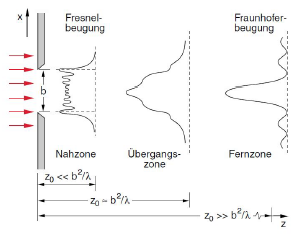
\includegraphics[width=0.9\textwidth]{abstande.png}
	\caption{Fresnel- und Frauenhofer Näherung. Im Fernfeld kann die Frauenhofer Näherung angewandt werden, wohingegen im Nahfeld die Fresnel Näherung angewandt wird. Entnommen aus \autocite{anleitung-ws2014}}
	\label{Theoriebild}
\end{figure}

In der Nahzone wird die Lichtausbreitung mithilfe der Fresnel-Näherung beschrieben. Diese gilt, wenn der Abstand des Beugungsobjekts zum Schirm klein ist. Ist dieser Abstand hingegen groß, also gilt $z_0 >> b$, wird das Beugungsbild mithilfe der Fraunhofer-Näherung für das Fernfeld beschrieben. Das elektrische Feld in der Fraunhofer-Näherung wird lässt sich mit \cref{eq:fraunhofer} bestimmen.

\begin{equation}
E\left( x', y', z'\right) = A\left( x', y', z'\right) \mathcal{F}\left( E_0\left( x, y, z_0\right) e^{i\Phi\left( x, y, z_0\right) }\right) \left( \nu_x, \nu_y\right) 
\label{eq:fraunhofer}
\end{equation}

Das Interferenzbild im Fernfeld entspricht also der Fouriertransformierten des Beugungsobjekts.

\subsection{Beugung am Gitter}
Bei der Beugung am Gitter entstehen nach dem Huygenschen Prinzip Kugelwellen, die mit einander interferieren. Die Interferenz ist entweder positiv bei einer Phasendifferenz von $2\pi$ oder negativ bei einer Phasendifferenz von $\pi$. Es entsteht also ein Beugungsbild, das vom Abstand zwischen Gitter und Schirm $d$, der Gitterkonstante $b$, der Spaltzahl $N$ und dem Beugungswinkel $\theta$ abhängig ist. Dies kann mit \cref{eq:beugung} berechnet werden.

\begin{equation}
I(\theta) = I_0 \text{sinc}^2\left( \frac{N\pi d \sin(\theta)}{\lambda}\right)  \text{sinc}^2\left( \frac{\pi b \sin(\theta)}{\lambda}\right) 
\label{eq:beugung}
\end{equation}

Um den Gitterabstand zu bestimmen, benötigt man allerdings nur die Bedingung für positive Interferenz. Sie lautet:

\begin{equation}
	k \lambda = b \sin(\theta); k\in \mathbb{N}_0
\end{equation}

\subsection{Optische Fouriertransformation mit Linsen}
In diesem Versuch soll hauptsächlich im Bereich der Fraunhofer-Näherung gearbeitet werden. Diese gilt aber erst im unendlichen. Daher wird eine Linse im Strahlengang positioniert, die das Bild der Fouriertransformierten in der Brennebene darstellt. Dieser Aufbau wird als 2f-Aufbau bezeichnet, da seine Länge der zweifachen Brennweite der Linse entspricht. Der Aufbau kann um eine weitere Linse erweitert werden, die eine Rücktransformation ausführt, um so wieder das ursprüngliche Bild zu erhalten. Die Linse wird dabei im Abstand $f$ von der Fourierebene positioniert. Im Abtand $f$ auf der anderen Seite der Linse wird dann das Objekt sichtbar. Der dazu nötige Aufbau ist in \cref{4f} dargestellt und wird 4f-Aufbau genannt.

\begin{figure}[h!]
	\centering
	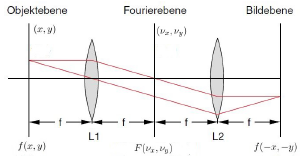
\includegraphics[width=0.9\textwidth]{4f.PNG}
	\caption{Schematische Darstellung des 4f-Aufbaus, der hier zur Fourierfilterung eingesetzt wird. Entnommen aus \autocite{anleitung-ws2014}}
	\label{4f}
\end{figure}

\subsection{Frequenzfilterung}
Mithilfe des 4f-Aufbaus kann nun eine Fourierfilterung durchgeführt werden. Hierfür können verschiedene Filter in der Fourierebene platziert werden. Ein Tiefpass wird dabei mithilfe einer Blende realisiert, die nur Licht in der Mitte der nullten Beugungsordnung durchlässt. Ein Hochpass wird mit einer Nadel erzeugt, die mittig in der Fourierebene platziert wird. Außerdem können auch bestimmte Frequenzen gefiltert werden, um periodisches Rauschen zu entfernen.

\subsection{Dunkelfeldmethode}
\label{Dunkelfeld}
Die Intensität eines Lichtfeldes, das Betragsquadrat des elektrischen Feldes kann auf einem Schirm mit bloßem Auge erkannt werden. Das elektrische Feld selbst ist allerdings nicht direkt sichtbar, da keine Informationen über die Phase des Felds bekannt sind. Um das elektrische Feld trotzdem zu detektieren, wird die Dunkelfeldmethode verwendet. Dazu nehmen wir an, dass das beugende Objekt dem elektrischen Feld eine ortsabhängige Phase aufprägt. Das E-Feld lässt sich nun schreiben als:

\begin{equation}
	E(x, y) = a e^{i\Phi\left( x, y\right) }.
\end{equation}

Für kleine Phasenänderungen gilt dann:

\begin{equation}
	E(x, y) = a\left( 1 + i\Phi\left( x, y\right) \right) .
\end{equation}

Fouriertransformiert ergibt sich dann:

\begin{equation}
	\mathcal{F}\left( E\left( x, y\right) \right)  = a\left( \delta\left( \nu_x\right) \delta\left( \nu_y\right) + \mathcal{F}\left( i\Phi\left( x, y\right) \right) \right) .
\end{equation}

Wird nun der erste Summand gefiltert, ergibt sich nach der Rücktransformation:

\begin{equation}
	\mathcal{F}^{-1}\left( \mathcal{F}\left( E\left( x, y\right) \right) \right) = E\left( x, y\right) = ia\Phi\left( x, y\right) .
\end{equation}

Die Intensität ist nun also abhängig von der Phase des elektrischen Feldes, somit ist die Phase auf dem Schirm sichtbar.

\section{Übergang von Nah- zu Fernfeld}
In diesem Versuchsteil wird das Beugungsbild eines Gitters in Abhängigkeit des Abstandes zwischen Schirm und Gitter beobachtet. Der schematische Aufbau, um diesen Sachverhalt zu untersuchen, ist in \cref{Lana1} zu sehen.
Dabei wird ein kollimierter Laserstrahl mit einer Wellenlänge von $\lambda = 633 nm$ auf einen Schirm gerichtet. 
\begin{figure}[h!]
	\centering
	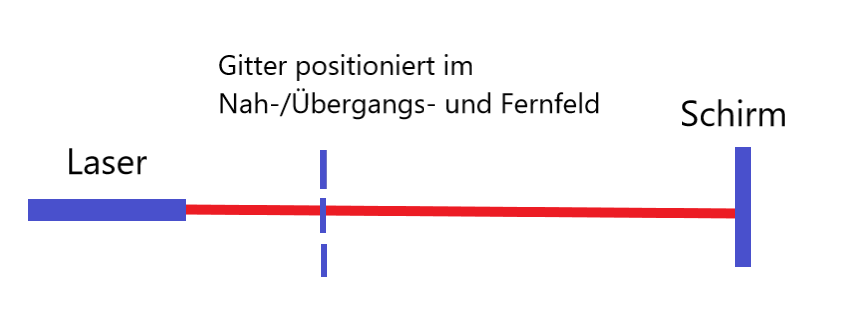
\includegraphics[scale = 0.65]{Lana-Bild1.png}
	\caption{Aufbau zur visuellen Bestimmung des Nah-/Übergans- und Fernfeldes. Dies ist ein skizzenhafter Aufbau des Versuchs.}
	\label{Lana1}
\end{figure}
Der Laserstrahl wird, um ihn zu kollimieren, auf eine Linse gerichtet.
Danach trifft der Laserstrahl auf ein Gitter, welches in verschiedenen Abständen vom Laser in den Strahlengang gebracht wird. Die Abstände zwischen Laser und Gitter variieren von 500mm und 3800mm. Auf dem Schirm kann ein Beugungsbild erkannt werden, welches mittels eines Intensitätsmessgerätes aufgenommen wird.
Mit diesem Aufbau kann nun das Beugungsbild bei unterschiedlichem Abstand zwischen Schirm und Gitter beobachtet werden. \cref{alle} zeigt den Verlauf der Beugungsbilder bei veränderlichem Abstand. Je größer der Abstand vom Schirm zum Gitter wird, desto kleiner wird der Abstand zwischen Gitter und Laser. Je näher sich das Gitter zum Laser bewegt, desto mehr wird sich das Fernfeld einstellen.
\begin{figure}[h!]
	\centering
	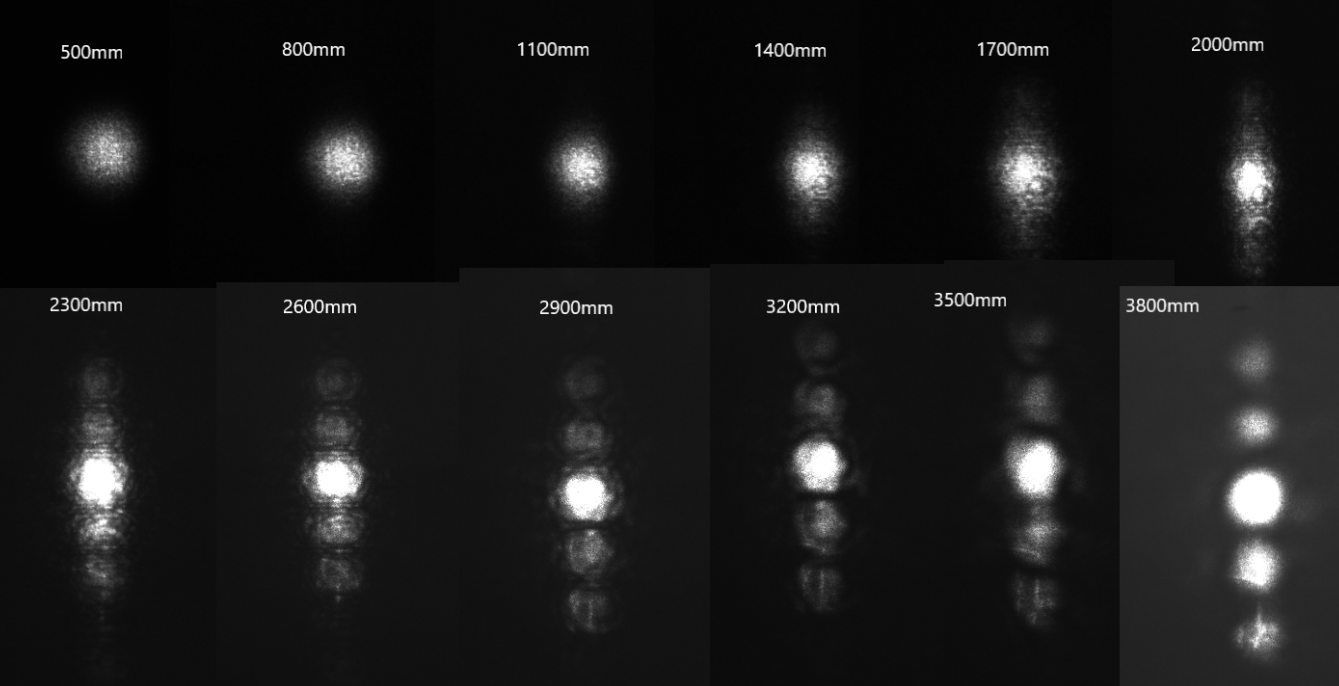
\includegraphics[scale = 0.65]{alleabstande.png}
	\caption{Es sind die Beugungsbilder in Abhängigkeit der Abstände zwischen Schirm und Gitter aufgetragen. Oben Links ist das Beugungsbild im Nahfeld zu erkennen bei einem Abstand von 500mm. Unten rechts ist das Beugungsbild im Fernfeld zu erkennen bei einem Abstand von 3800mm. Von oben links nach unten rechts nimmt der Abstand zu. Der Abstand nimmt in 300mm Abständen zu.}
	\label{alle}
\end{figure}
In \cref{alle} kann in einem Abstand von $500 mm$ bis $1400 mm$ das Nahfeld erkannt werden. Bei einem Abstand von $1700 mm$ bis $2600 mm$  kann das Übergangsfeld beobachtet werden und in einem Abstand von $2900 mm$ bis $3800 mm$ kann das Fernfeld beobachtet werden. Die angegebenen Grenzen sind keine scharfen Grenzen. Häufig kann man an den Grenzen beide Effekte erkennen. Die Effekte sind beim Nah- und Fernfeld vor allem an den Rändern sichtbar (also bei $500 mm$ bzw. bei $3800 mm$) und beim Übergangsfeld bei einem Abstand von $2000 mm$. Diese Angaben wurden mit \cref{Theoriebild} erhoben. Gründe für diese Einteilung sind, dass sich die Maxima höherer Ordnung erst im Fernfeld klar unterscheiden lassen und sich die Maxima im Nahfeld in einem Punkt treffen. Charakteristisch für die Übergangszone ist das vermischen beider Effekte. Das Hauptmaximum ist deutlich zu erkennen, jedoch gibt es entfernt vom Hauptmaximum noch Helligkeitserscheinungen, die nach außen hin abschwächen und kaum zu erkennende Peaks ausbilden. Diese Charakteristiken können im Vergleich von \cref{Theoriebild} und \cref{alle} an den oben genannten Bildern beobachtet werden.


\section{Gitterkonstanten ohne Linse}
In diesem Abschnitt wurden die Gitterkonstanten verschiedener Gitter bestimmt. Dafür wurde das Gitter in den Strahlengang gestellt. Die Kamera wird $\SI{3800}{mm}$ entfernt positioniert. Dieser Aufbau ist in \cref{aufbaugitter} dargestellt.

\begin{figure}[h]
	\centering
	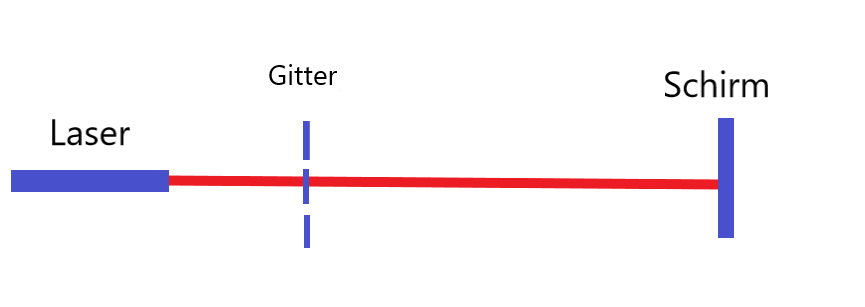
\includegraphics[width=0.9\textwidth]{Lana-Bild2.png}
	\caption{Schematischer Aufbau des Versuchs zur Bestimmung der Gitterkonstanten}
	\label{aufbaugitter}
\end{figure}

Die dabei aufgenommenen Bilder sind in \cref{gitterfernfeld} zu sehen. Man erkennt deutlich, dass die Abstände zwischen den einzelnen Punkten von links nach rechts größer werden. Außerdem sind die Bilder links eher unscharf, nach rechts werden die einzelnen Punkte schärfer und lassen sich besser unterscheiden. Bei allen Gittern wird nun der Abstand zwischen dem nullten Beugungsmaximum und dem ersten und zweiten Beugungsmaximum nach oben und unten ermittelt. Dazu wird ein Lineal verwendet, dass auf den unbearbeiteten Bildern mit fotografiert wurde und so als Skala dient. Eine Ausnahme bildet das zweite Beugungsmaximum nach oben bei Gitter 2, dieses konnte nicht identifiziert werden. 

\begin{figure}
	\centering
	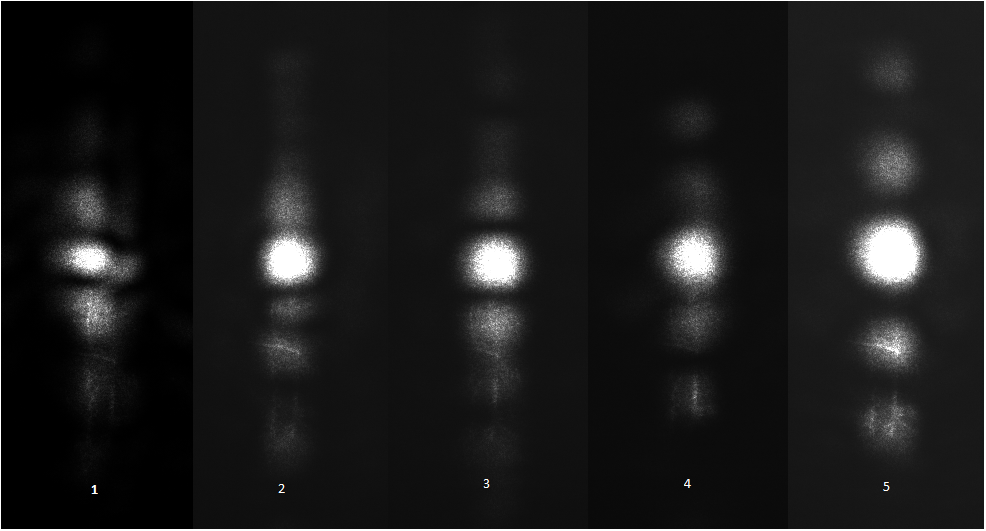
\includegraphics[width=0.9\textwidth]{gitter_fernfeld.png}
	\caption{Die Beugungsbilder der 5 Gitter von Gitter 1 ganz links bis Gitter 5 ganz rechts, aufgenommen ohne Linse}
	\label{gitterfernfeld}
\end{figure}

Aus dem Abstand der einzelnen Beugungsmaxima zum nullten Beugungsmaximum $a$ und dem Abstand zwischen Gitter und Kamera $d$ kann dann mit \cref{eq:sin} $\theta$ für jedes Beugungsmaximum einzeln bestimmt werden.

\begin{equation}
	\theta = \arctan\left(\frac{a}{d}\right)
	\label{eq:sin}
\end{equation}

Nun lässt sich die Gitterkonstante des untersuchten Gitters mit \cref{eq:gk} bestimmen, mit $k$ der Nummer des Beugungsmaximums.

\begin{equation}
	k\lambda = b \sin(\theta)
	\label{eq:gk}
\end{equation}

Bei jedem Gitter, außer dem zweiten aus oben genanntem Grund, wurde die Gitterkonstante jeweils viermal bestimmt, mit den beiden ersten Beugungsmaxima nach oben und unten ausgehend vom nullten Maximum. Aus diesen wurde dann der Mittelwert gebildet. Die Ergebnisse sind in \cref{tab} zusammengefasst.

\begin{table}[h]
	\caption{Die Gitterkonstanten der fünf untersuchten Gitter in mm}
\begin{tabular}{lllll}
	Gitter 1 & Gitter 2& Gitter 3& Gitter 4& Gitter 5\\
	 $0,386\pm0,048$ & $0,456\pm0,053$ & $0,363\pm0,041$ & $0,323\pm0,032$ & $0,252\pm0,020$
\end{tabular}
\label{tab}
\end{table}

Wie bereits in \cref{gitterfernfeld} erkennbar, wird die Gitterkonstante bei kleinerer Gitternummer kleiner. Das wurde auch schon während dem Versuch mit bloßem Auge so abgeschätzt. Eine Ausnahme bildet Gitter 1, welches kleiner ist als Gitter 2.
Die Unsicherheit beim Ablesen der Abstände wurde auf $\SI{\pm1}{mm}$ geschätzt. Daraus ergibt sich mithilfe der Formel für die Fehlerfortpflanzung (\cref{eq:utheta}) die Unsicherheit von $\theta$ und daraus mit \cref{eq:ugk} die Gesamtunsicherheit der Gitterkonstanten.

\begin{align}
u(\theta) &= \frac{u(a)*d}{a^2 +d^2}
\label{eq:utheta}\\
u(b) &= \frac{u(\theta) k \lambda \cos(\theta)}{sin(\theta)^2}
\label{eq:ugk}
\end{align}

Auch die Unsicherheiten wurden für jedes Beugungsmaximum einzeln bestimmt, anschließend wurde daraus der in der Tabelle aufgeführte Mittelwert gebildet.

\section{Gitterkonstanten mit Linse}
Im nächsten Schritt wurde die Gitterkonstante erneut bestimmt, allerdings mit leicht verändertem Versuchsaufbau (dargestellt in \cref{aufbaugitter2}). Nun ist hinter dem Gitter im Abstand von $\SI{1150}{mm}$ eine Linse positioniert. Diese fokussiert das Licht auf den Schirm, der wiederum im Abstand von $\SI{1150}{mm}$ zur Linse positioniert ist.

\begin{figure}[h]
	\centering
	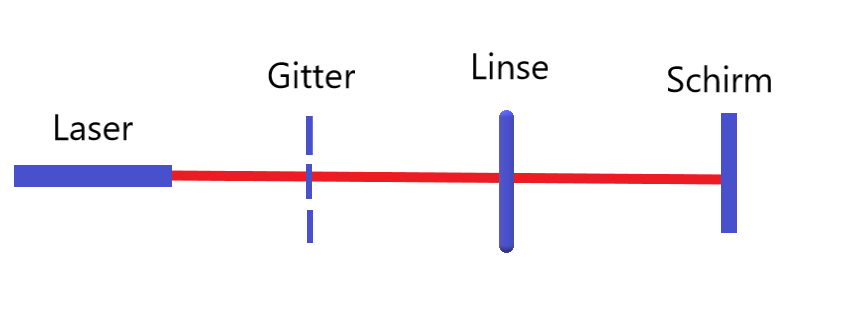
\includegraphics[width=0.9\textwidth]{Lana-Bild3}
	\caption{Schematischer Aufbau des 2. Versuchs zur Bestimmung der Gitterkonstanten.}
	\label{aufbaugitter2}
\end{figure}

Die dabei entstandenen Beugungsbilder sind in \cref{gitterfourier} zu sehen. Auch hier ist deutlich erkennbar, dass die Beugungsmaxima bei höherer Gitternummer weiter auseinander liegen. Erneut wird beobachtet, dass die Beugungsmaxima bei höherer Gitternummer schärfer und besser unterscheidbar sind, während die Bilder bei niedriger Gitternummer unscharf und die Beugungsmaxima schwer trennbar sind. Dieser Effekt ist hier deutlich stärker ausgeprägt als bei der Messung ohne Linse.
Die Abstände werden hier genauso bestimmt wie oben beschrieben, mit dem Lineal als Skala. Bei Gitter 3-5 wurden wieder das erste und zweite Beugungsmaximum in beide Richtungen zur Rechnung verwendet. Bei Gitter 1 und 2 waren diese nicht identifizierbar, hier wurden in beide Richtungen die ersten Maxima verwendet, die von der weiß leuchtenden Fläche rund um das nullte Beugungsmaximum als getrennte Punkte erkennbar waren. Dies war in allen vier Fällen das vierte Beugungsmaximum. Um welches Maximum es sich bei diesen Gittern handelt, konnte visuell nicht herausgefunden werden. Es ist aber wahrscheinlich, dass es sich um das Vierte handelt, da bei dieser Wahl die Gitterkonstanten von Gitter 2 aus beiden Messungen ungefähr übereinstimmen. Da Gitter 1 eine größere Gitterkonstante als Gitter 2 haben muss, muss es sich beim für die Rechnung verwendeten Beugungsmaximum mindestens um das Vierte handeln, höhere Ordnungen sind aber theoretisch auch möglich.

\begin{figure}[h]
	\centering
	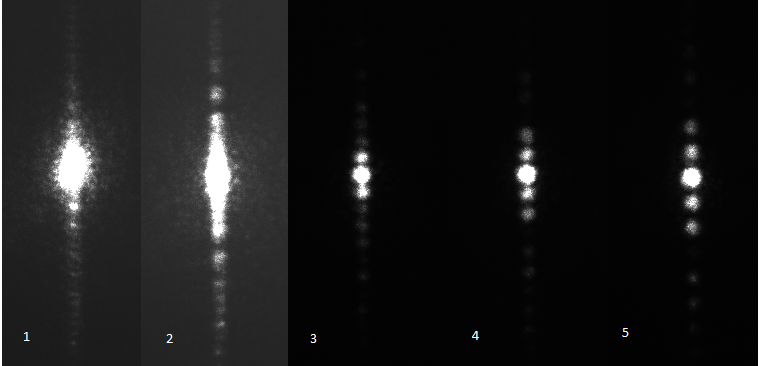
\includegraphics[width=0.9\textwidth]{gitter_fourier.png}
	\caption{Die Beugungsbilder der 5 Gitter von Gitter 1 ganz links bis Gitter 5 ganz rechts, aufgenommen mit Linse.}
	\label{gitterfourier}
\end{figure}

Zur Berechnung der Gitterkonstanten wurden wie im vorigen Abschnitt \cref{eq:sin} und \cref{eq:gk} verwendet, anschließend wurde aus diesen Werten der Mittelwert gebildet. Die Unsicherheiten wurden wieder mit \cref{eq:utheta} und \cref{eq:ugk} und anschließender Bildung des Mittelwerts bestimmt. Aufgrund der deutlich besseren Bildqualität wurden die Unsicherheit beim Ablesen für Gitter 3-5 auf $\SI{\pm0,5}{mm}$ geschätzt Die Ergebnisse beider Messreihen sind in \cref{tab2} zusammengefasst.

\begin{table}[h]
	\caption{Die Gitterkonstanten der fünf untersuchten Gitter in mm, ohne Linse und mit Linse.}
	\begin{tabular}{llllll}
		&Gitter 1 & Gitter 2& Gitter 3& Gitter 4& Gitter 5\\
		Mit Linse&$0,683\pm0,080$ & $0,485\pm0,081$ & $0,377\pm0,072$ & $0,332\pm0,057$ & $0,269\pm0,037$\\
		Ohne Linse&$0,386\pm0,048$ & $0,456\pm0,053$ & $0,363\pm0,041$ & $0,323\pm0,032$ & $0,252\pm0,020$
	\end{tabular}
	\label{tab2}
\end{table}

Die Werte für die Gitterkonstante sind bei allen Gittern (außer Gitter 1) innerhalb der angegebenen Unsicherheiten gleich. Damit kann die Messung als Erfolg gewertet werden. Die Gitterkonstanten lassen sich offenbar auf beide Arten gut bestimmen. Der einzige abweichende Wert ist die Gitterkonstante von Gitter 1 bei Messung ohne Linse. Hierfür sind mehrere Erklärungen möglich. Zum einen weicht das Beugungsbild für dieses Gitter deutlich von den anderen ab, die Punkte sind stark verschwommene Figuren, die nicht als Punkte erkennbar sind. Dies erschwert die Bestimmung des Abstandes zwischen den Beugungsmaxima und damit die Bestimmung der Gitterkonstante. Zum anderen ist es möglich, dass es sich bei den beobachteten Maxima nicht um die ersten bzw. zweiten Maxima handelt, sondern um höhere Ordnungen. Dann müssten dafür müssten andere niedrigere Beugungsmaxima so miteinander verschwimmen, das eine visuelle Trennung nicht mehr möglich ist. Dies kann aufgrund er schlechten Bildqualität nicht ausgeschlossen werden.

\section{Fourierfilterung}
\subsection{Fourier Schriftzug}
Im weiteren Versuchsverlauf sind alle Experimente nach dem 4-f-Aufbau realisiert, der in \cref{4f-Aufbau} zu sehen ist. Zuerst soll ein „Fourier“ Schriftzug vor einem Gitter modelliert werden, indem das Gitter entfernt wird.

\begin{figure}[h]
	\centering
	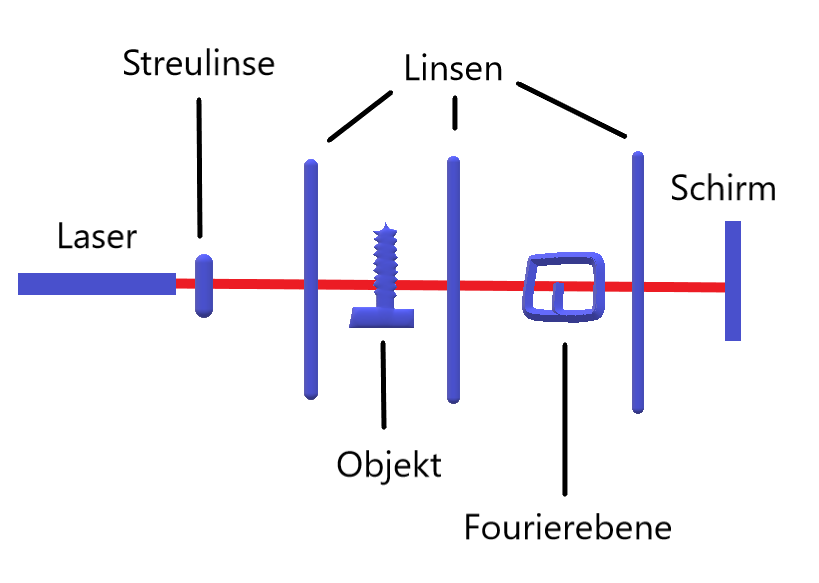
\includegraphics[width=0.8\textwidth]{Lana-Bild4}
	\caption{Schematischer Aufbau des der Fourierfilterung.}
	\label{4f-Aufbau}
\end{figure}


Dazu wird eine Tiefpassfilterung benutzt, da die im Vergleich große Schrift hauptsächlich aus niedrigen Frequenzen besteht. 


\begin{figure}[h]
\begin{subfigure}[c]{0.5\textwidth}

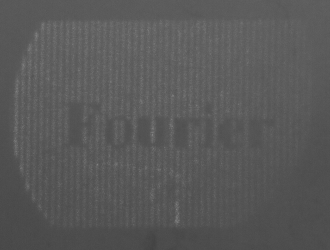
\includegraphics[width=0.9\textwidth]{Fourier.png}
	      \caption{}
          \label{fig:NiceImage1}
          
\end{subfigure}
\begin{subfigure}[c]{0.5\textwidth}
	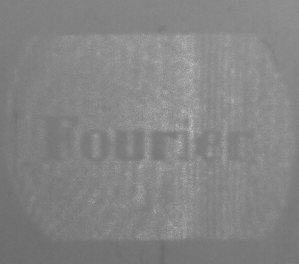
\includegraphics[width=0.9\textwidth]{Fourier_Filter.png}
	      \caption{}
          \label{fig:NiceImage2}
\end{subfigure}
\caption{In \cref{fig:NiceImage1} ist der "Fourier" Schriftzug ohne Filter zu sehen; in \cref{fig:NiceImage2} mit einem Tiefpassfilter.}
\label{Fourier}
\end{figure}   

In \cref{Fourier} ist zu sehen, wie sich der Tiefpassfilter auf das Bild auswirkt. Das Gitter ist zum größten Teil nicht mehr als solches zu erkennen. Allerdings konnten die Linien nicht vollständig entfernt werden. Das liegt höchstwahrscheinlich daran, dass der Filter nicht perfekt in der Fourierebene lag, dadurch können verschiedene Effekte auftreten, wie z.B. ein gewisse räumliche Verzerrung. 

\subsection{Nenner eines Bruches entfernen}
Daraufhin soll der Nenner eines $\frac{1}{2}$ Bruchs entfernt werden. Wie in \cref{fig:Bruch} zu sehen ist, befindet sich unter dem Zähler ein Gitter, welches sich nicht bei dem Nenner befindet. Es werden also praktisch beide Zahlen entfernt, allerdings ist durch das Gitter immer noch der Umriss der 1 sichtbar. Dieses entfernen geschieht durch eine Hochpassfilterung, was bedeutet, dass niedrige Frequenzen entfernt werden. Das hat funktioniert, da in \cref{fig:Bruch_filter} die Zwei, also der Nenner nicht mehr erkennbar ist.

\begin{figure}[h]
	\begin{subfigure}[c]{0.5\textwidth}
		
		\includegraphics[width=0.6\textwidth]{Bruch.png}
		\caption{}
		\label{fig:Bruch}
		
	\end{subfigure}
	\begin{subfigure}[c]{0.5\textwidth}
		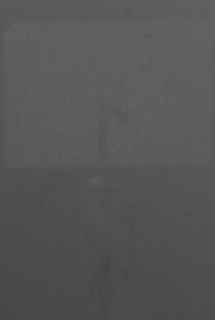
\includegraphics[width=0.58\textwidth]{Filter_Bruch.png}
		\caption{}
		\label{fig:Bruch_filter}
	\end{subfigure}
	\caption{In \cref{fig:Bruch} ist der $\frac{1}{2}$ Bruch ohne Filter zu sehen; in \cref{fig:Bruch_filter} mit einem Hochpassfilter, wodurch die Zwei entfernt wurde und die eins als negativ zu erkennen bleibt.}
	\label{Bruch}
\end{figure}   

\newpage

\subsection{Tiefpassfilterung bei einem Quadratgitter}
Als nächstes soll ausprobiert werden, was passiert, wenn ein Quadratgitter eingesetzt wird, das mit einem eindimensionalem Tiefpassfilter in verschiedenen Ausrichtungen gefiltert wird. Das ungefilterte Bild ist in \cref{fig:Gitter} zu sehen. Dazu im Vergleich wurde in \cref{fig:0Gitter} ein Tiefpassfilter im Winkel von 0° Grad eingebaut. Da der Tiefpass alle Frequenzen außer denen, die im 0° Winkel sind durchgelassen. Deshalb wurde erwartet, dass die Linien orthogonal zum Frequenzbild erkennbar sind. Allerdings ist das besonders am Rand und zum Teil auch in der Mitte des Bildes nicht immer deutlich zu erkennen. 

Ähnliche Probleme gibt es auch in \cref{fig:45Gitter} und \cref{fig:90Gitter}, in denen der Tiefpassfilter jeweils um 45° und 90° gedreht sind. Besonders in \cref{fig:45Gitter} lässt sich die Ausrichtung nur noch erahnen, während bei der 90° Drehung das Muster nur in der Mitte des Bildes unterbrochen wird.

Diese hellen Strahlen, die sich an der räumlichen Ausrichtung des Filters orientieren und damit die erwarteten Muster unterbrechen, stammen höchstwahrscheinlich daher, dass der Tiefpassfilter sich beim Messen nicht perfekt in der Fourierebene befand. Trotzdem lässt sich bei genauerem Hinschauen das erwartete Muster erkennen.





\begin{figure}[ht]
	\begin{subfigure}[c]{0.5\textwidth}
		
		\includegraphics[width=1\textwidth]{Quadratgitter.png}
		\caption{}
		\label{fig:Gitter}
		
	\end{subfigure}
	\begin{subfigure}[c]{0.5\textwidth}
		\includegraphics[width=1\textwidth]{0Grad_Tiefpass_quadrat.png}
		\caption{}
		\label{fig:0Gitter}
	\end{subfigure}


	\begin{subfigure}[c]{0.5\textwidth}
		
		\includegraphics[width=1\textwidth]{45Grad_Tiefpass_quadrat.png}
		\caption{}
		\label{fig:45Gitter}
		
	\end{subfigure}
	\begin{subfigure}[c]{0.5\textwidth}
		\includegraphics[width=1\textwidth]{90Grad_Tiefpass_quadrat.png}
		\caption{}
		\label{fig:90Gitter}
	\end{subfigure}
	\caption{In \cref{fig:Gitter} ist das Quadratgitter ohne einen Filter zu sehen; in \cref{fig:0Gitter} mit einem Tiefpassfilter im 0° Winkel,in \cref{fig:45Gitter} im 45° Winkel und in \cref{fig:90Gitter} im 90° Winkel.}
	\label{blabla}
\end{figure}  



\newpage

\subsection{Hochpassfilterung einer Schraube}
Daraufhin wird eine Schraube einer Hochpassfilterung unterzogen. In \cref{Schraube} sind die Bilder mit und ohne Filter zu sehen. In \cref{fig:Schraube_Filter} ist dabei nur noch der Umriss der Schraube zu sehen. Da sowohl der Laser selbst als auch die Schraube selbst nahezu homogen sind, werden dafür fast nur niedrige Frequenzen benutzt. Der Rand der Schraube hat allerdings mehre kleine Kanten, die durch hohe Frequenzen dargestellt werden und deshalb durch den Hochpassfilter durchkommen.

\begin{figure}[h]
	\begin{subfigure}[c]{0.5\textwidth}
		
		\includegraphics[width=1\textwidth]{Schraube_ohneFilter.png}
		\caption{}
		\label{fig:Schraube}
		
	\end{subfigure}
	\begin{subfigure}[c]{0.5\textwidth}
		\includegraphics[width=1\textwidth]{Schraube.png}
		\caption{}
		\label{fig:Schraube_Filter}
	\end{subfigure}
	\caption{In \cref{fig:Schraube} ist die Schraube ohne Filter zu sehen, in \cref{fig:Schraube_Filter} wurde noch ein Hochpassfilter benutzt.}
	\label{Schraube}
\end{figure}  


\newpage

\subsection{Dunkelfeldmethode}
Zuletzt soll noch die Dunkelfeldmethode getestet werden, die Luftströme sichtbar machen
kann. Die Theorie dazu ist in \cref{Dunkelfeld} beschrieben. Um den Versuch auszuführen wird ein Teelicht in den Strahlengang eingesetzt und der Laser so justiert,
dass er sich etwas über der Flamme befindet. Nach dem Einsetzen eines Hochpassfilters,
lassen sich die Luftströme sichtbar machen. Diese Luftströme, die durch das Erhitzen der
Luft durch das Teelicht entstehen, entsprechen dabei den hellen Stellen in Abb. 9. Dies
ist der Fall, da die Luftströme eine Änderung der Phase verursachen und damit durch
die Hochpassfilterung sichtbar gemacht werden.

\begin{figure}[h!]
	\centering
	\includegraphics[scale = 1]{Flamme.png}
	\caption{Anwendung der Dunkelfeldmethode. Die helle Stelle zeigt einen Luftstrom, der
		durch das Teelicht entstanden ist.}
	\label{Flamme}
\end{figure}


\newpage

\section{Zusammenfassung}



Die Überlegungen aus der Theorie für den ersten Versuchsteil haben sich im  Experiment qualitativ bestätigt. Es konnten die charakteristischen Eigenschaften von Fern- Übergangs- und Nahfeld beobachtet werden.

Auch der zweite Versuchsteil kann als Erfolg gewertet werden. Die Gitterkonstanten der fünf Gitter konnten sowohl ohne Linse bei großem Abstand zwischen Gitter und Schirm als auch mit Linse, wobei der Schirm in der Brennebene der Linse platziert wurde, bestimmt werden. Nur für Gitter 1 stimmen die beiden berechneten Werte nicht überein. Insgesamt erscheinen die berechneten Werte plausibel, die Abnahme der Gitterkonstante für höhere Gitternummern konnte schon während dem Versuch mit bloßem Auge festgestellt werden.




Außerdem hat die Filterung der verschiedenen Objekte funktioniert. Es wurde zwar in einigen Fällen deutlich, dass die jeweiligen Filter sich nicht perfekt in der Fourierebene befunden haben, allerdings konnten trotzdem alle grundsätzlichen Ziele erreicht werden. Ein Problem war allerdings, dass nur ein Bild von der Dunkelfeldmethode gemacht wurden, sodass sich nicht gut zeigen lässt, dass es sich tatsächlich um Luftströme gehandelt hat. Außerdem fehlt ein Vergleichsbild ohne die Kerze. 
